\chapter{Experimental Setup}
\section{RHIC}
The Relativistic Heavy Ion Collider (RHIC) is a superconducting charged hadron collider located at Brookhaven National Labs (BNL) in Upton, NY, United States. RHIC is capable of accelerating heavy ions such as Au (gold) or Cu (copper) nuclei to energies of 200 GeV per nucleon. RHIC is also capable of accelerating lighter ions such as protons, deuteron, and helium to 200 GeV per nucleon and 510 GeV per nucleon in the case of protons. The machine has been demonstrated to reliably create so called QGP matter at temperatures in excess of seven trillion degrees Fahrenheit.

There are two major detector experiments currently operating in interaction regions around the RHIC ring: PHENIX and STAR. A typical operation schedule for RHIC is to run the accelerator for five and a half months every year in what is called a "Run". There have been 16 "Runs" so far but the relevant run for this thesis was Run 15 taken in 2015 which ran proton colliding with gold ions (p+Au) at 200 GeV per nucleon for part of its running.

\begin{figure}[!h]
\begin{center}
\includegraphics[width=0.65\linewidth]{figs/rhic-map.png}
\caption{A helicopter's view of the accelerator chain in BNL starting at the Tandems (in gold) and ending at the RHIC ring (in blue). STAR and PHENIX can be seen at two of the interaction regions. The ring is 2.38 miles in length.}
\end{center}
\end{figure}

RHIC is at the end of a chain of smaller accelerators that are used to "feed" the ions into RHIC, where they are accelerated (or decelerated in some circumstances) to the desired collision energy. For heavy ions such as Au, the process is listed in detail below \cite{ROSER200223}.
\begin{enumerate}
  \item{} A pulsed sputter Au ion source generates negative ions in the Tandem Van De Graaff.
  \item{} The ions are passed through an electron stripping foil to achieve a positive 12 charge and accelerated to 1 MeV per nucleon.
  \item{} The ions pass through magnets to further strip electrons and filter charge, yielding to a positive 32 charge state.
  \item{} The ions are sent to the Booster Synchrotron which accelerates them to 95 MeV per nucleon and leaves them at a positive 77 charge.
  \item{} The ions enter the Alternating Gradient Synchrotron (AGS) in 24-ion bunches. The ions are debunched and rebunched into four bunches and then accelerated to 10.8 GeV per nucleon.
  \item{}  The bunches then exit the AGS one at a time, where their Au ions are stripped of their two remaining electrons, yielding a final charge state of positive 79. Finally, the bunches are transferred to their respective buckets in RHIC . 
\end{enumerate}

For protons, the process instead begins at the the Linear Accelerator (LINAC) facility. The protons are then sent through the chain of accelerators in a similar way to the heavy ions until reaching RHIC in either a polarized or unpolarized state. 

Once the ions have reached RHIC, they will enter one of two independent rings, blue or yellow, each circulating in an opposite direction. The ions in the rings are deflected and focused by 1,740 superconducting magnets using niobium-titanium conductors. Once the ions are focused and accelerated to the desired parameters around the RHIC, the ions are deflected into the six interactions regions where the blue and yellow rings intersect to produce collisions. It is at these interaction regions where the major experiments have set up their detectors, with STAR at the 6 o'clock position and PHENIX at the 8 o'clock position.

The time period of which the collisions continue is known as a fill, and the average length of a fill is eight hours. As the fill wears on, the collision rate substantially decreases as the density of ions in the machine decreases. Once the collision rate has been reduced sufficiently, it is more cost efficient to start the fill over at a higher collision rate.  

For this thesis, the relevant dataset is p+Au 200 GeV Run 15 taken in 2015. Specific details about this dataset are found in section \ref{Run 15}.

%Electron cooling was implemented in RHIC to increase the luminosity of fills and slow the luminosity decay. The basic concept of electron cooling is to shoot electrons at the heavy ion beams in RHIC 
%\begin{figure}[!h]
%\begin{center}
%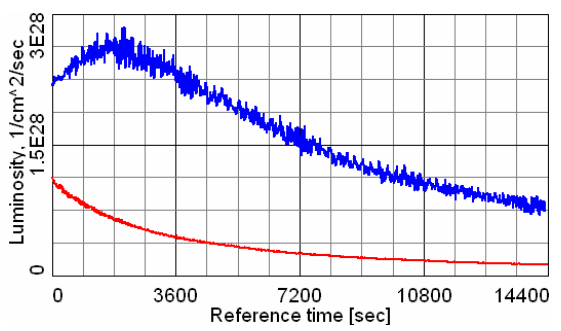
\includegraphics[width=0.5\linewidth]{figs/rhic_electron_cooling_sim.png}
%\caption{The luminosity vs time for Au-Au at 200 GeV simulations with (blue) and without (red) electron cooling. Electron cooling is shown to be an effective way of increasing luminosity in simulations. ~\cite{fedotov2007progress}}
%\end{center}
%\end{figure}

\section{PHENIX}
PHENIX, the Pioneering High Energy Nuclear Interaction eXperiment, came online in 2000 along with RHIC and is located at the 8 o'clock interaction region along the RHIC ring. PHENIX is one of the two major RHIC experiments along with STAR, the Solenoidal Tracker At RHIC. PHENIX detector philosophy differs from STAR in that PHENIX makes use of more than a dozen independent detector subsystems of roughly equal experimental weight whereas STAR makes use of only four with its Time Projection Chamber (TPC) being the primary detector. 

PHENIX's detectors throughout the years include (in no particular order) the Drift Chamber (DC), the Pad Chambers (PC), the Ring Imaging Cherenkov (RICH), the Hadron Blind Detector (HBD), the Time Expansion Chamber (TEC), the Time of Flight (TOF), the Electromagnetic Calorimeter (EMCAL), the Muon Tracker (MuTr), the Muon Identifier (MuID), the Muon Piston Calorimeter (MPC), the Muon Piston Calorimeter Extension (MPC-EX), the Beam-Beam Counter (BBC), the Zero Degree Calorimeter (ZDC), the Forward Calorimeter (FCAL), the Multiplicity and Vertex Detector (MVD), the Reaction Plane Detector (RPD), the Resistive Plate Chambers (RPC), the Silicon Vertex Detector (VTX), and the Forward Silicon Vertex Detector (FVTX). For this thesis, the relevant detectors installed in 2015 are the DC, PC, RICH, BBC, and FVTX. The DC, PC, and RICH are located in the mid-rapidity region relative to collisions (Central Arms) and the BBC and FVTX are located in the forward (and backward) rapidity region relative to collisions (Forward Arms) \cite{Adcox2003469}. 

PHENIX makes use of the three powerful magnets in order to bend charged the particles' trajectories: the Central Magnet (CM), the North Muon Magnet (MMN), and the South Muon Magnet (MMS). For this thesis, the relevant magnet is the CM. 

PHENIX makes use of a state of the art Data Acquisition System (DAQ) which is capable of writing 400 MB/s of information to disk. More details about the PHENIX DAQ are found in section \ref{PHENIX DAQ}.
\begin{figure}[!h]
\begin{center}
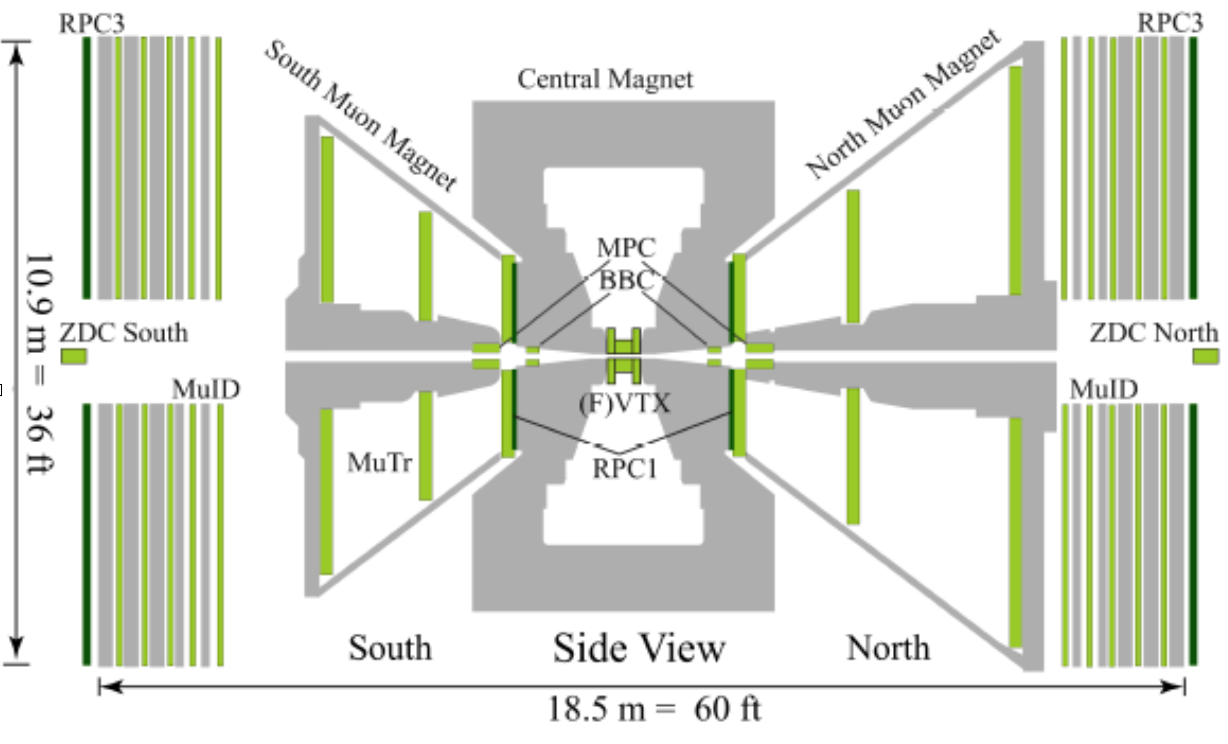
\includegraphics[width=0.5\linewidth]{figs/phenix_schematic.png}
\caption{The top is a cross section diagram of the PHENIX detector from the incoming beam's perspective. The bottom is a cross section diagram of the PHENIX detector from the top down. The central arm detectors are not present in the bottom diagram. }
\end{center}
\end{figure}

\begin{figure}[!h]
\begin{center}
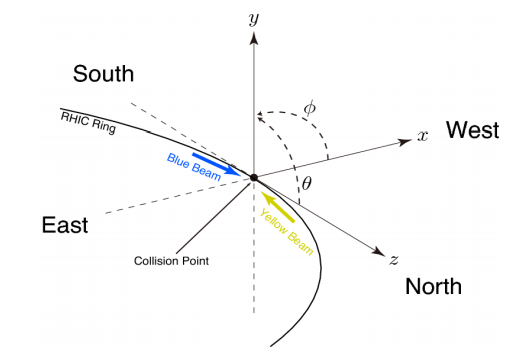
\includegraphics[width=0.55\linewidth]{figs/phenix_coord.png}
\caption{The PHENIX coordinate system. The origin is in the middle of the PHENIX detector at the collision point. North and south are parallel to beam axis. East and west are transverse to the beam axis. Central detectors have a west and an east arm on either side of the beam. Forward detectors have a north and a south arm relative to the origin.}
\end{center}
\end{figure}

\subsection{Forward Rapidity Detectors}
\subsubsection{Beam Beam Counter}
The BBC is a forward detector used to determine the event start time, vertex, centrality, and event plane. The BBC is composed of two mirror image arrays, a South and a North Arm, that surround the beam pipe 144 cm on opposite sides of the nominal collision point just behind the Central Magnet, covering $3.0 < |\eta| < 3.9$ and 2$\pi$ radians in azimuth. Each BBC arm is made of 64 elements each composed of a 3-cm length quartz Cherenkov radiator connected to a 2.5 cm diameter Hamamatsu R6178 mesh dynode PMT (photomultiplier tube), as shown in Fig \ref{fig:bbc_dector}. The outer and inner diameters of the BBC are 30 cm and 10 cm, respectively.% allowing for a 1 cm clearance of the beam pipe.
\begin{figure}[!h]
\begin{center}
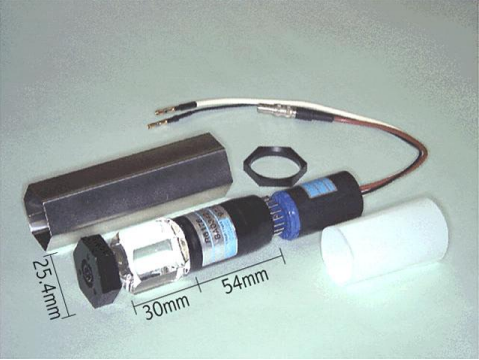
\includegraphics[width=0.5\linewidth]{figs/bbc_pmt.png}
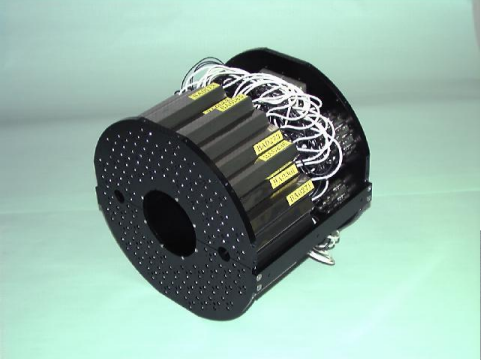
\includegraphics[width=0.5\linewidth]{figs/bbc_arm.png}
\caption{Photographs of the BBC detector. The left is of a single detector element consisting of a quartz Cherenkov and a PMT. The right is of one of the BBC arms, consisting of 64 detector elements.}\label{fig:bbc_dector}
\end{center}
\end{figure}

The BBC has a timing resolution of 52�4 ps. The BBC is used to mark the event start time for the entire PHENIX detector by averaging the emitted particles arrival time at each BBC arm. The timing difference between each arm provides an estimate of the collision's z-vertex by
\begin{equation}
z = c \frac{T_S - T_N}{2},
\end{equation}
where $T_S, T_N$ are the particle's arrival times for each arm and c is the speed of light.
In typical Au+Au 200 GeV collisions the BBC z-vertex resolution is 0.5 cm. This rough estimate of the vertex is used during triggering. Specific details about triggers are in section \ref{PHENIX DAQ}.
%The BBC also provides the centrality classification, as defined in chapter 2, of a collision event in PHENIX. 

%\begin{figure}[!h]
%\begin{center}
%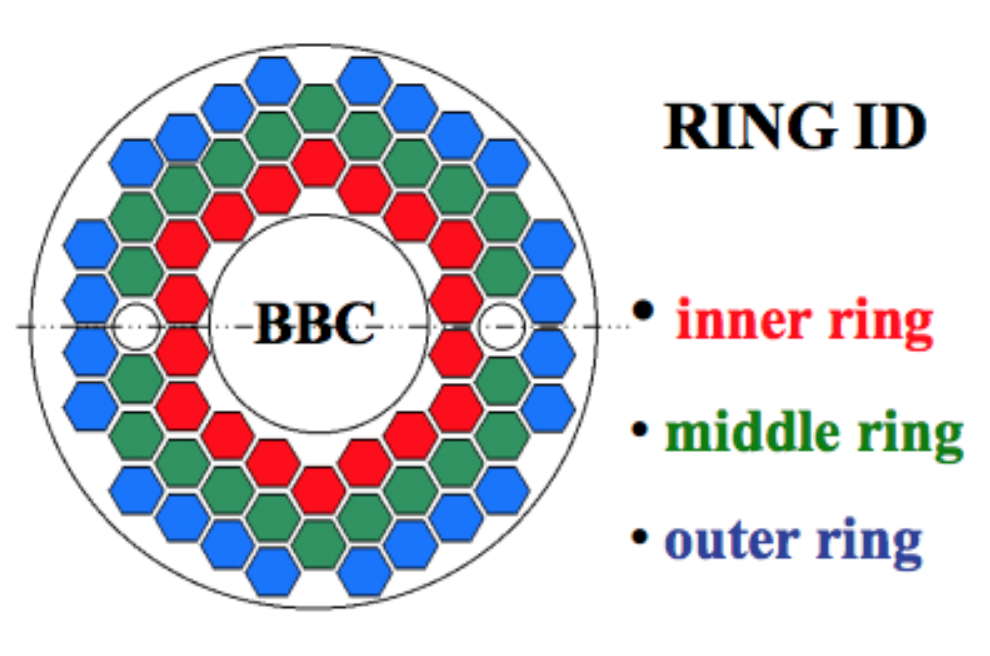
\includegraphics[width=0.4\linewidth]{figs/bbc_ring_schematic.png}
%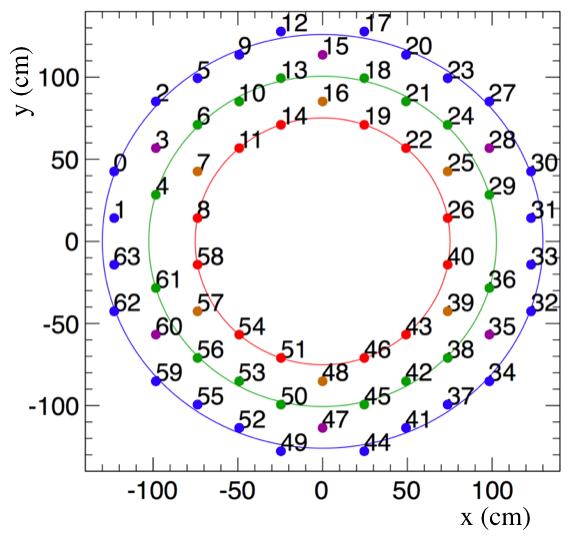
\includegraphics[width=0.4\linewidth]{figs/bbc_rings.png}
%\caption{TBA}
%\end{center}
%\end{figure}
%[LIST PHENIX forward rapidity detectors (muon ID, muon tracker, muon trigger, FVTX, RPC (maybe forget about the big list)]
\subsubsection{Forward Vertex Detector}
%[talk about how it is a new upgrade in 2012, talk about ]
The FVTX is a PHENIX detector upgrade which became operational for physics data taking in 2012. The FVTX uses include charged particle tracking, collision vertex determination, and event plane determination \cite{Aidala201444}. The FVTX consists of two identical endcaps covering a combined psuedorapidity range of 1 $<|\eta|<$ 3 and full azimuth coverage. Each endcap has four stations of silicon mini-strip sensors with a pitch of 75 $\mu m$ arranged in the radial direction around the beam pipe. The basic unit of construction is a wedge that has a silicon strip sensor and read-out chips. There are four FVTX layers in each endcap.
\begin{figure}[h!]
\begin{center}
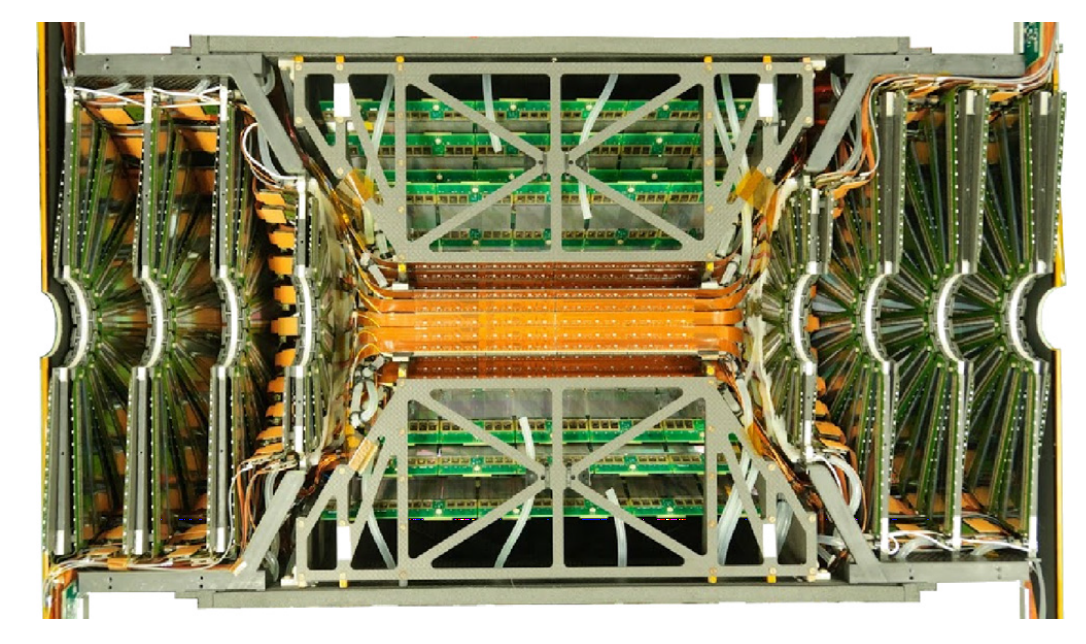
\includegraphics[width=0.45\linewidth]{figs/fvtx_cutaway.png}
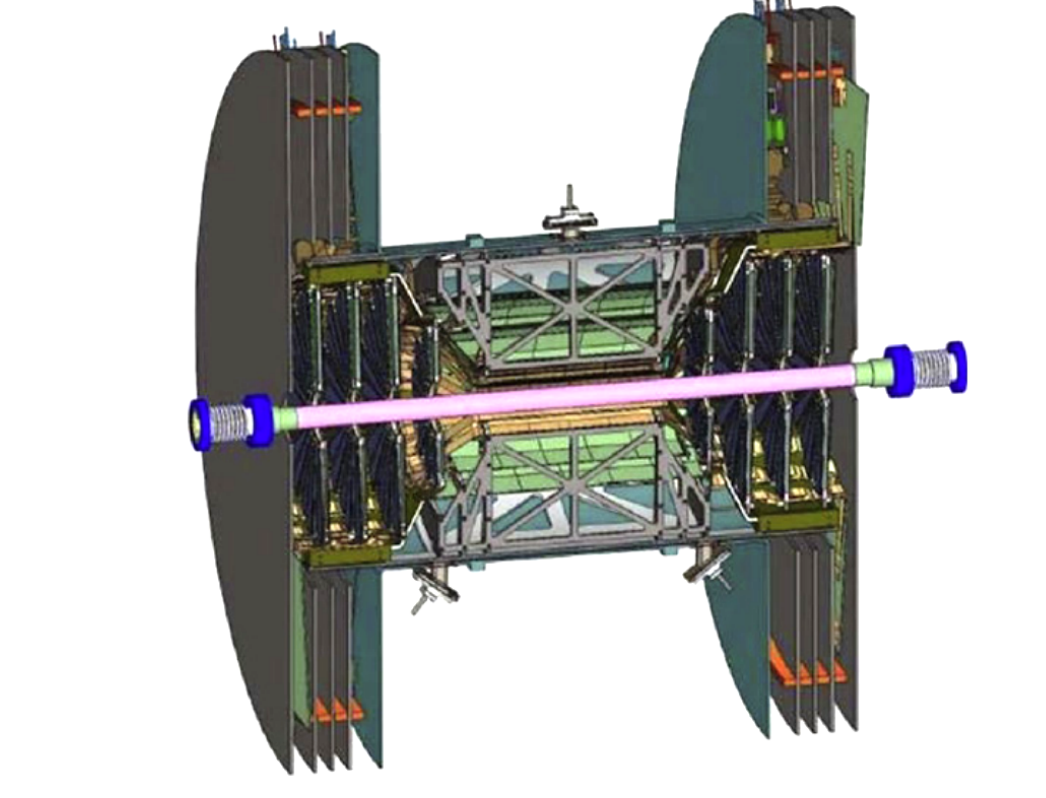
\includegraphics[width=0.45\linewidth]{figs/fvtx_diagram.png}
\caption{The left is a photograph of half of the FVTX. The FVTX are the half disks on either end of the picture. The FVTX is only 20 cm in the z direction from the PHENIX coordinate system origin (the center of the picture. The right is a schematic of the FVTX at a slightly different angle. }\label{fig:fvtx_cutaway}
\end{center}
\end{figure}
%\subsubsection{FVTX Clustering}
\subsection{Midrapidity Detectors}
\subsubsection{Drift Chamber}
The DC consists of two gas multi-wire chambers, one located in each arm. The DC is used to measure particle trajectories in the r $\phi$ plane.
The DC is the innermost subsystem in the central arms, located ~2 m from the z-axis, placing it in a residual magnetic field of 0.6 kiloGauss from the CM. Apart from the VTX, the DC is the first detector encountered by a particle in mid-rapidity. 

As a charged particle passes through the DC volume, the gases are ionized to create free electrons. These electrons cause a chain reaction of ionizations which are measured by an anode wire. The DC is designed in such a way that the drift velocities of the elections are predicable enough to relate time and position together. 

\begin{figure}[!h]
\begin{center}
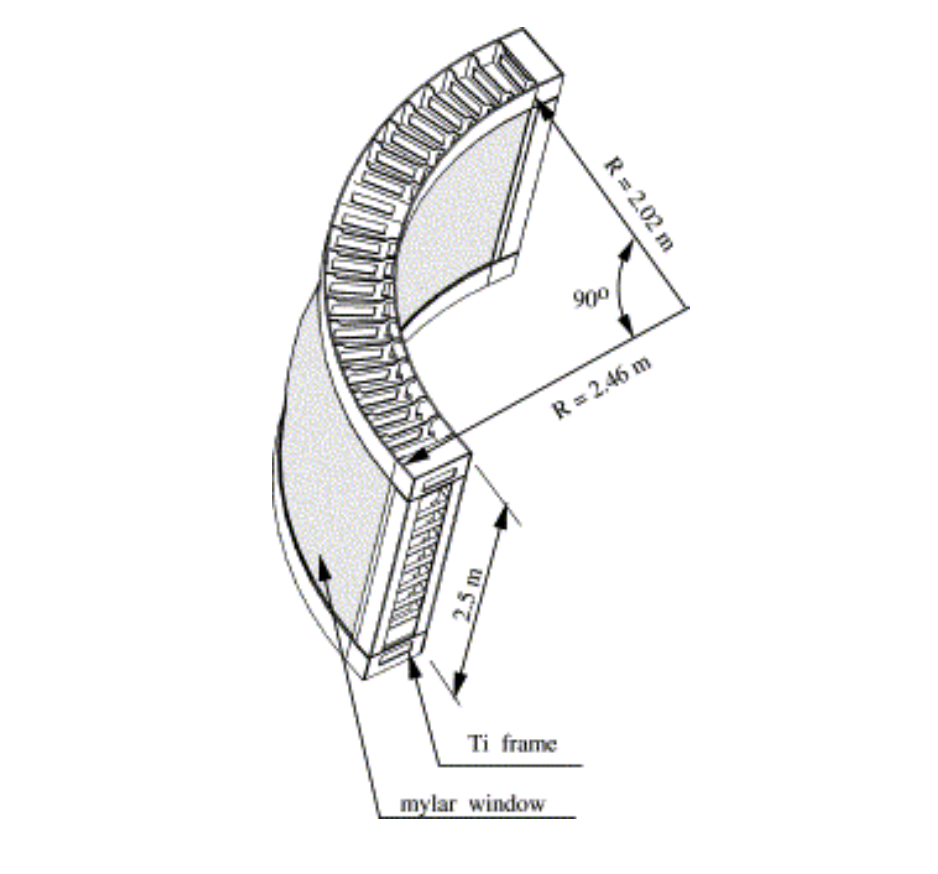
\includegraphics[width=0.55\linewidth]{figs/dc_diagram.png}
\caption{A diagram of the DC titanium frame which encloses the detector.}\label{fig:dc_diagram}
\end{center}
\end{figure}

Each identical DC arm is cylindrical in design and covers 2.5 m along the beam direction and is 0.4 m thick as seen Fig \ref{fig:dc_diagram}. A gas mixture of $50\%$ Argon and $50\%$ Ethane is used in each arm of the DC. Each arm is divided into 20 equal sectors covering 4.5 degrees in $\phi$. Each sector contains six types of wire modules stacked radially and labeled X1, U1, V1, X2, U2, V2, respectively from the inside out. The X wires run parallel to the beam to perform precise four $\phi$ measurements while the U and V wires are set at small angles of about six degrees relative to the X wires to provide information about the z position of the track. A diagram of the wire layout in each sector is shown in Figure \ref{fig:dc_wire_diagram}. In total, the DC consists of 6500 anode wires leading to 13,000 readout channels, with a measured single wire resolution of 165 �m and a spatial resolution of  2 mm.
\begin{figure}[!h]
\begin{center}
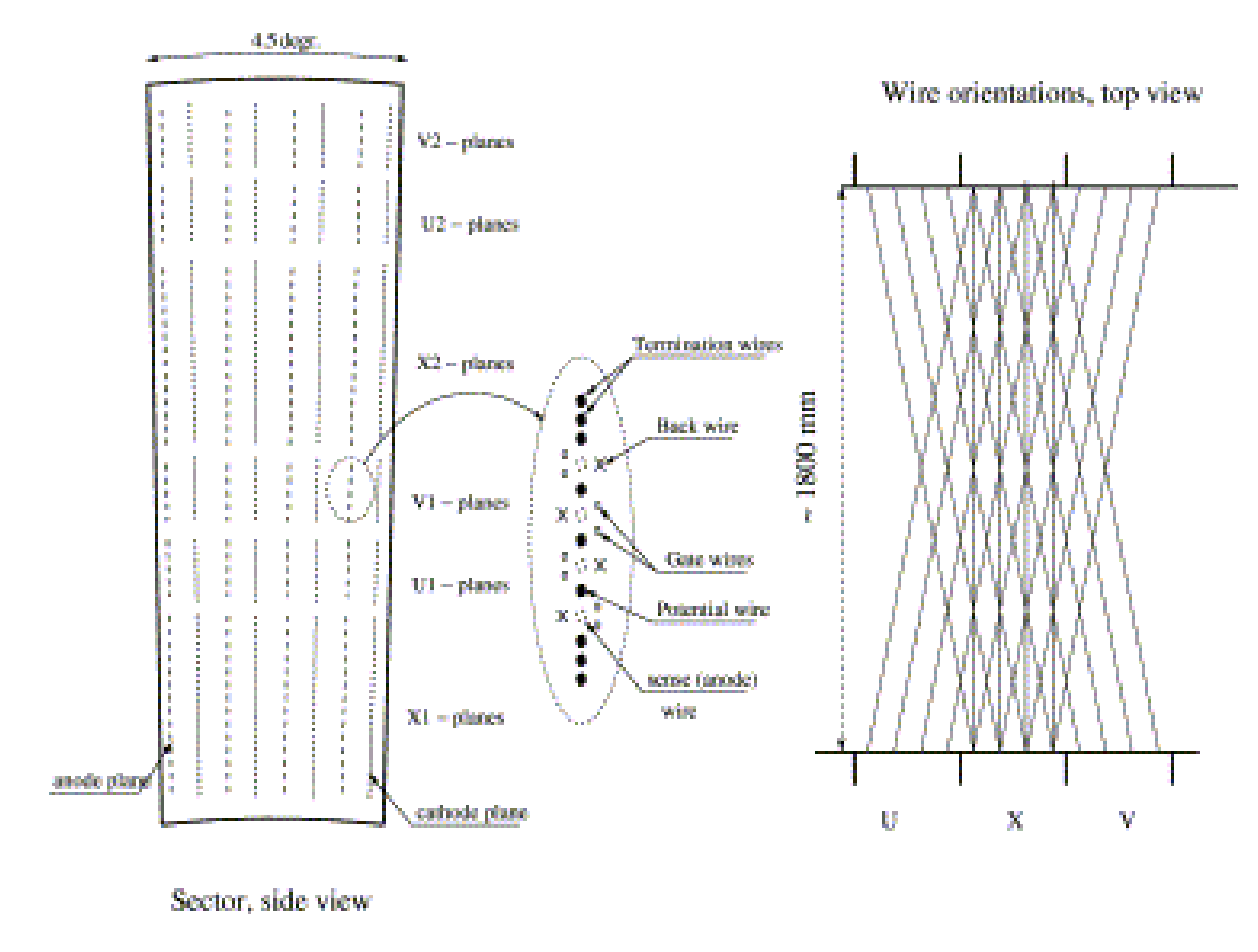
\includegraphics[width=0.55\linewidth]{figs/dc_wire_diagram.png}
\caption{A diagram of the X, U, and V wires in the DC.}\label{fig:dc_wire_diagram}
\end{center}
\end{figure}

\subsubsection{Pad Chambers}
The PCs are multi-wire proportional chambers which consist of three separate layers of detectors measuring precise hit positions and making up the bulk of the PHENIX tracking system. The innermost layer, PC1, is located in both the East and West arms immediately outside the DC, providing a measurement of the z position at the back plane of the DC. The second layer, PC2, is located behind the RICH in the West arm only. The outer layer, PC3, is in both arms and provides a second point on the straight line trajectories of the tracks through the detector, outside of the magnetic field.
\subsubsection{Ring Imaging Cherenkov Detector}
The RICH detector is located immediately behind the PC1 and provides the primary electron identification for PHENIX. The RICH consists of two identical detectors located in each arm and provides e over $\pi$ discrimination below the pion Cherenkov threshold of 4.65 GeVc in the CO2 gas used in the detectors.
\subsubsection{Electromagnetic Calorimeter}
The EMCAL is the outermost subsystem in the central arms and is designed primarily to measure the energies and positions of photons and electrons. It also plays a key role in the identification of as well as providing triggering for rare events. Two different EMCAL designs were utilized with 6 sectors based on a lead-scintillator design and 2 sectors based on a lead-glass design. The two different designs were chosen deliberately as each provides advantages and disadvantages, for instance the lead glass has a better energy resolution, while the lead scintillator has better linearity and timing.
\subsection{PHENIX Data Acquisition System}
\label{PHENIX DAQ}
PHENIX makes use of a fast DAQ to manage the transfer and collation of hundreds of kB of event data from over two dozen independent detector subsystems at a rate of over 6 kHz. This amounts to writing to disk hundreds of MB/s, something which the PHENIX DAQ consistently achieves for months of around the clock use. 

The collection of a  Granule Timing Module (GTM), Front End Modules (FEM), and a Data Collection Modules (DCM) is known as a granule and is the minimal combination of DAQ hardware sufficient for data production as shown in Fig \ref{fig:granule_diag}. Each detector subsystem's output data is managed by a granule. Pipelined Field ProGrammable Arrays (FPGA) with carefully controlled dead time are used to calculate the trigger decisions. The FPGAs are fed information from the experiment. Once the FPGAs compute the trigger decision, the trigger signals are monitored by the GTM. If trigger decision is positive, the GTMs instruct the FEMs to release their data from their buffers and send them to their graunules' DCM. If the decision is negative, otherwise the FEMs are instructed to dump the data.  Once the DCM is instructed to send its data downstream, it is sent to the event builder which will be discussed in an upcoming section.

\subsubsection{Triggering}
PHENIX has the capability of running 128 independent triggers, in practice only 32 are used. Each of the triggers have a scale down number to control the relative bandwidth each trigger receives. To understand the PHENIX triggers, it is useful to learn about the beam clock.

The PHENIX trigger is tied to the clock of the blue beam, one of the two counter circulating rings of which RHIC is comprised. The clock rate is fixed at 9.38 MHz and is tied to the rate at which RHIC overlaps bunches of ions in the interaction regions. Every time a bunch of ions from the blue ring overlap with a bunch of ions from the yellow ring, there is a blue clock trigger. This clock is stable by necessity of the precision required to run a complex accelerator like RHIC. This blue clock trigger is the backbone of PHENIX triggering for there can be no ion collision event if there is no overlap of bunches. Consequently, almost every PHENIX trigger is AND'd with the clock trigger.

The trigger which is given the largest bandwidth is the minimum bias (minbias) trigger. As the name suggests, the trigger seeks to mark the detection of an ion collision while reducing the any bias to the type of the collision to a minimum. To achieve this, data from the BBC and ZDC are used, although the ZDC is less relevant than the BBC for defining the trigger. Although what constitutes a minbias observation varies with collision species, the BBC minbias trigger is generally defined as $>$0 PMTs in each arm above threshold. Not only is this condition a good indication that a ion collision occurred, it is also the minimum information necessary to calculate the collision vertex position using the BBC. The vertex information is important because it is used to select for collisions which occur in the narrow range of acceptance of current PHENIX detector configuration. This range is -10 cm $< z<$ 10 cm where z is defined in the PHENIX coordinate system in fig (TBA). For completeness, PHENIX takes BBC minbias triggers with z vertex cuts of � 30 cm and with no vertex cut. The collection of all these triggers is what is considered to be the PHENIX minbias trigger.

In Run 15, a unique high multiplicity trigger was implemented to enhance event statistics for events producing the most amount of particles. This trigger consisted of requiring at least 35 out of 64 PMTs in the south arm of the BBC. More details about this trigger are located in section \ref{Run 15}.
\begin{table}[h!]
\centering
\caption{An example Run15 p+Au 200 GeV relevant trigger configuration and parameters. A trigger's scale down number reduces its rate by 1/(1+scale down). }%numbers from run435737
    $\begin{array}{|c|c|c|c|c|}
    \hline 
    %\toprule
    %Collision Species & p+p & p+Au & units & a \\ \hline
    Trigger\thinspace Name & Scale\thinspace down & Trigger\thinspace rate & Vertex\thinspace cut & Part\thinspace of\thinspace minbias \\ \hline
     Clock & 196077 & 45 Hz  & N/A & no \\ \hline
    BBC(>0\thinspace PMTs)  & 100 &  695 Hz & � 10 cm & yes\\ \hline
    BBC(>0\thinspace PMTs)  & 2083 & 88 Hz & � 30 cm & yes\\ \hline
    BBC(>0\thinspace PMTs) & 3959 &94 Hz  &no\thinspace cut & yes\\ \hline
    BBC(>35\thinspace  PMTs) & 1 & 1640 Hz & � 10 cm & no \\ \hline
    \end{array}$
\end{table}

\begin{figure}[h!]
\begin{center}
\label{fig:granule_diag}
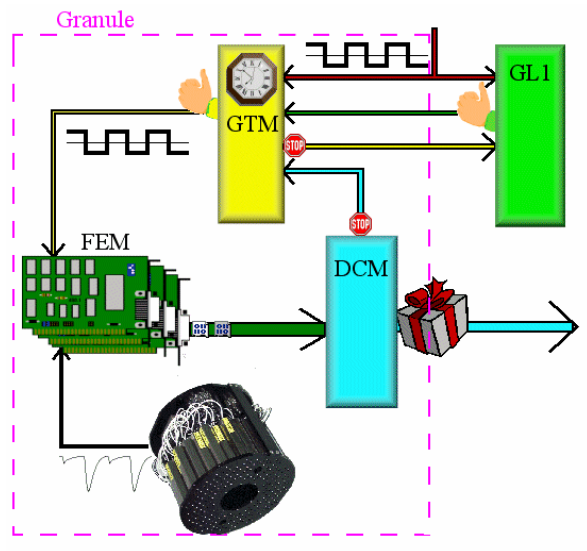
\includegraphics[width=0.55\linewidth]{figs/granule_diagram.png}
\caption{Diagram of a granule. Granules are the building blocks of the PHENIX DAQ. Each detector subsystem has at least one granule.} %Also, the GL1 has a granule.}
\end{center}
\end{figure}

%\begin{figure}
%\begin{center}
%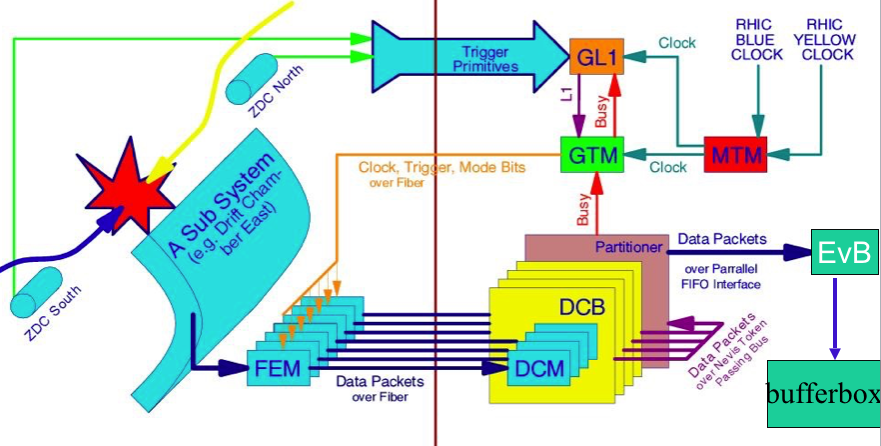
\includegraphics[width=0.75\linewidth]{figs/DAQ_diagram.png}
%\caption{Diagram of the .}
%\end{center}
%\end{figure}

\subsubsection{Event Builder}
Following the PHENIX DAQ downstream, after a positive trigger decision has been sent to each of the granules, the granules' data packets are sent to the event builder. It is the event builder's job to associate each granule's data packet from the same collision event into one bundle of data known as an event. The event builder consists of Sub Event Buffers (SEB), Assembly Trigger Processors (ATP), an Event Builder Controller (EBC), and a Gigabit Ethernet Switch as the communication management. Fig \ref{fig:evb_diag} provides a diagram of how these components are connected.

Granules send the data packets to the specific SEB assigned to that granule. The EBC receives global trigger information and assigns each ATP a specific collision event. The ATP then requests the data from all of the SEBs for the specific event assigned to it by the EBC. Once the ATP is successful, it writes the assembled event to disk and the EBC instructs the SEBs to flush the buffer for that event.
%This is more difficult than it may appear because event buffering means there will be multiple packets from each granule from different collision events.

\begin{figure}[h!]
\begin{center}
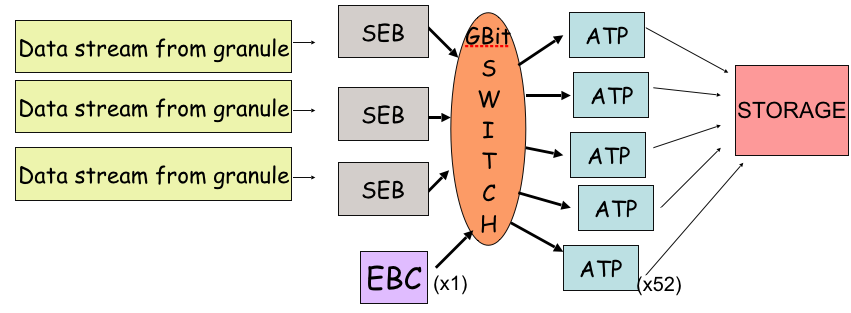
\includegraphics[width=0.73\linewidth]{figs/evb_diagram.png}
\caption{Diagram of the event builder. }\label{fig:evb_diag}
\end{center}
\end{figure}


%\subsubsection{Triggering}

\subsection{Run 15}
\label{Run 15}
Run 15 is the RHIC running period in the year 2015  which marks fifteen consecutive years of RHIC running since the year 2000. Run 15 began in January 2015 and ended in June of 2015. There were approximately eleven weeks of research viable, polarized p+p collisions at $sqrt{s}=$ 200 GeV, approximately 5 weeks of research viable polarized p+Au collisions at $\sqrt{s}=$ 200 GeV, and approximately one week of research viable p+Al collisions $sqrt{s}=$ 200 GeV. Of interest to this thesis are the p+p and p+Au datasets. 
\begin{table}[h!]
\caption{Some relevant RHIC parameters from Run 15.}
\begin{center}
    \begin{tabular}{| l | l | l | l |}
    \hline
    Collision Species & p+p & p+Au & units\\ \hline
    Total Particle Energy & 100.2 & 103.9 + 100.0  & GeV/nucleon \\ \hline
    Ions per Bunch & 225 &  225 + 1.6 & number $\times10^{9}$ \\ \hline
    Number of Bunches & 111& 111 & number\\ \hline
    Luminosity Average Per Fill& $63\times10^{30}$ & $45 \times10^{28}$&$cm^{-2}s^{-1}$ \\ \hline
    Total Delivered Luminosity & 382  & 1.27 & $pb^{-1}$ \\ \hline
    Average Fill Lifetime & 8 & 7 & hours\\ \hline
    \end{tabular}
\end{center}
\end{table}

In addition to providing the min-bias trigger for Run 15, the BBC was used to implement a high-multiplicity trigger in order to enhance the amount of the top $5\%$ highest multiplicity events. The high-multiplicity trigger requires 35 of the 64 BBC south arm PMTs to be above threshold in a given event to be satisfied. The relevant BBC arm for p+Au is the south arm since that is the Au-going direction so the multiplicity is much higher in the south arm. The enhancement can be seen in Figure \ref{fig:pau_centrality_trig}. 

%Also, the BBC was used to determine the event centrality by summing the charge collection of each
%BBC element; it is assumed the larger the charge collection the more central the
%event. This will be further discussed in Sec. (TBA) Moreover, the BBC can measure
%event plane using. For further BBC event plane calculation details see section (TBA).

\begin{figure}[h!]
\begin{center}
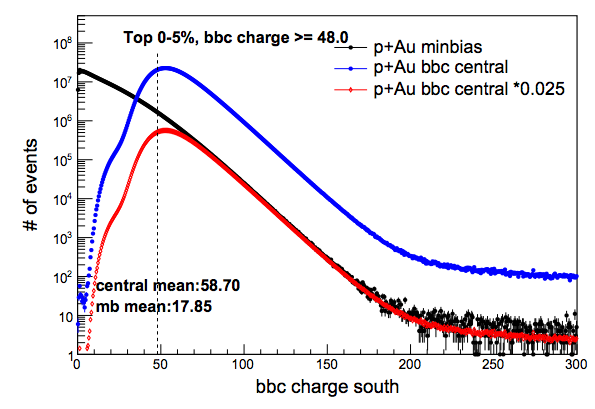
\includegraphics[scale=0.55]{figs/pAu_centrality_trigger.png}
\end{center}
\caption{The distribution of BBC charges in p+Au 200 GeV events for different triggers. The black curve is the distribution of charges for the minbias trigger. The blue and red curves are the distributions of charges for the high multiplicity trigger. The red curve being scaled by a factor of 1/40 to show agreement with with the black curve. The definition of the top 5\% more central events are BBC south charges $>=$ 48.0. The plot shows the large enhancement of the number of 0-5\% centrality events that are gained using the high multiplicity trigger compared to the number of 0-5\% centrality from the minbias trigger alone.}\label{fig:pau_centrality_trig}

\end{figure}

\subsubsection{Beam Collision Geometry}
For Run 15 p+Au 200 GeV running, RHIC's blue and yellow beams were not in perfect accordance to the PHENIX coordinate system. This was manifested in two separate ways.
First of all, the collision vertex is significantly offset from the z-axis to which all of the PHENIX detectors are aligned. This is a typical situation in PHENIX datasets but it must be addressed. The other effect, and the more significant of the two, comes from the fact that the beams are colliding at an angle of 3.6 milli-Radians in the x-z plane as illustrated in Fig \ref{fig:beam_angle}. This is a result of configuring RHIC magnets for the specific charge to mass ratios of the p+Au collision species.
The collision vertex in x and y is known as the beam center. The beam center varies over the course of data taking but its values on average are $(x,y) = (0.206,0.065) (cm)$. The distribution of z-vertices from collision events can be see in Fig \ref{fig:bbc_z_vtx_dist}. Due to the fact that the beams are colliding at an angle in the x-z plane, the x-component of the beam center will have a z-vertex dependence with a slope of -0.0036 cm of x per 1 cm of z.
Apart from how the beam angle effects the beam center values, it also violates the expectation of a uniform $\phi$ distribution of particles with respect to PHENIX detectors. PHENIX detectors are designed and aligned with respect to the PHENIX coordinate system with the expectation of geometric symmetry. A significant beam collision angle with respect to PHENIX detectors would be equivalent to PHENIX detectors being tilted which would violate geometric symmetry.
The physics analysis described in this thesis is sensitive to these beam geometry effects. A discussion on how to account for these effects will be in chapter 4.

% The reason a non-ideal beam geometry 
%creates an east west v2 measurement difference is because of the assumption that event plane angle is azimuthally
% isotropic during the event plane flattening calibration. In the translated and rotated frame where the beams aligned with the z-axis the event plane distribution would be %uniform, but in the lab frame the event plane distribution in $\phi$ would have regions of enhancement and reduction.
\begin{figure}[h!]
\begin{center}
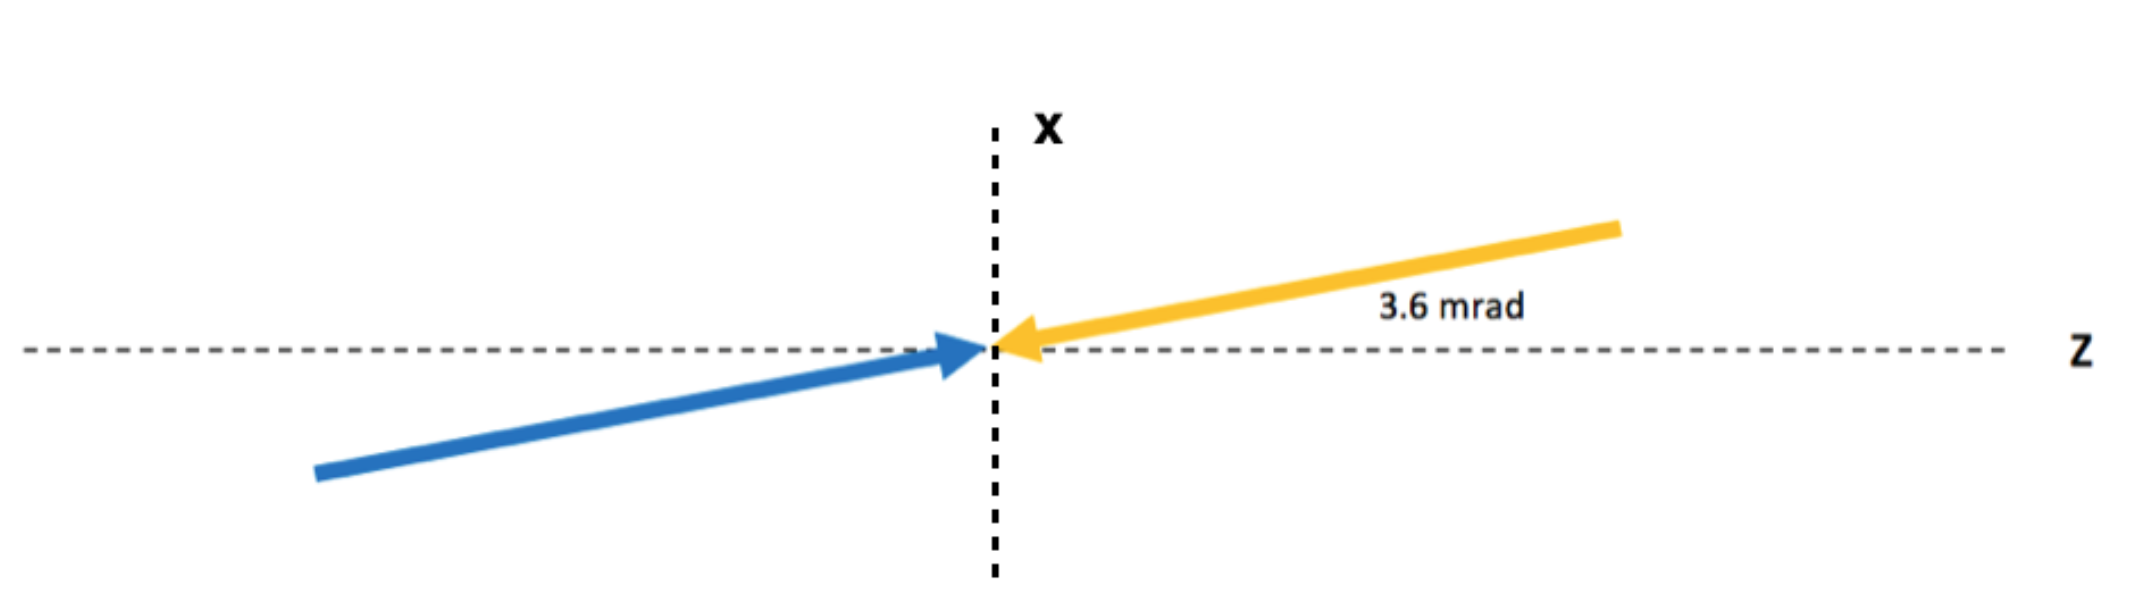
\includegraphics[width=0.85\linewidth]{figs/beam_angle.png}
\caption{A vector diagram illustrating the yellow and blue beam angle confirmation relative to the PHENIX coordinate system.}\label{fig:beam_angle}

\end{center}
\end{figure}

\begin{figure}[h!]
\begin{center}
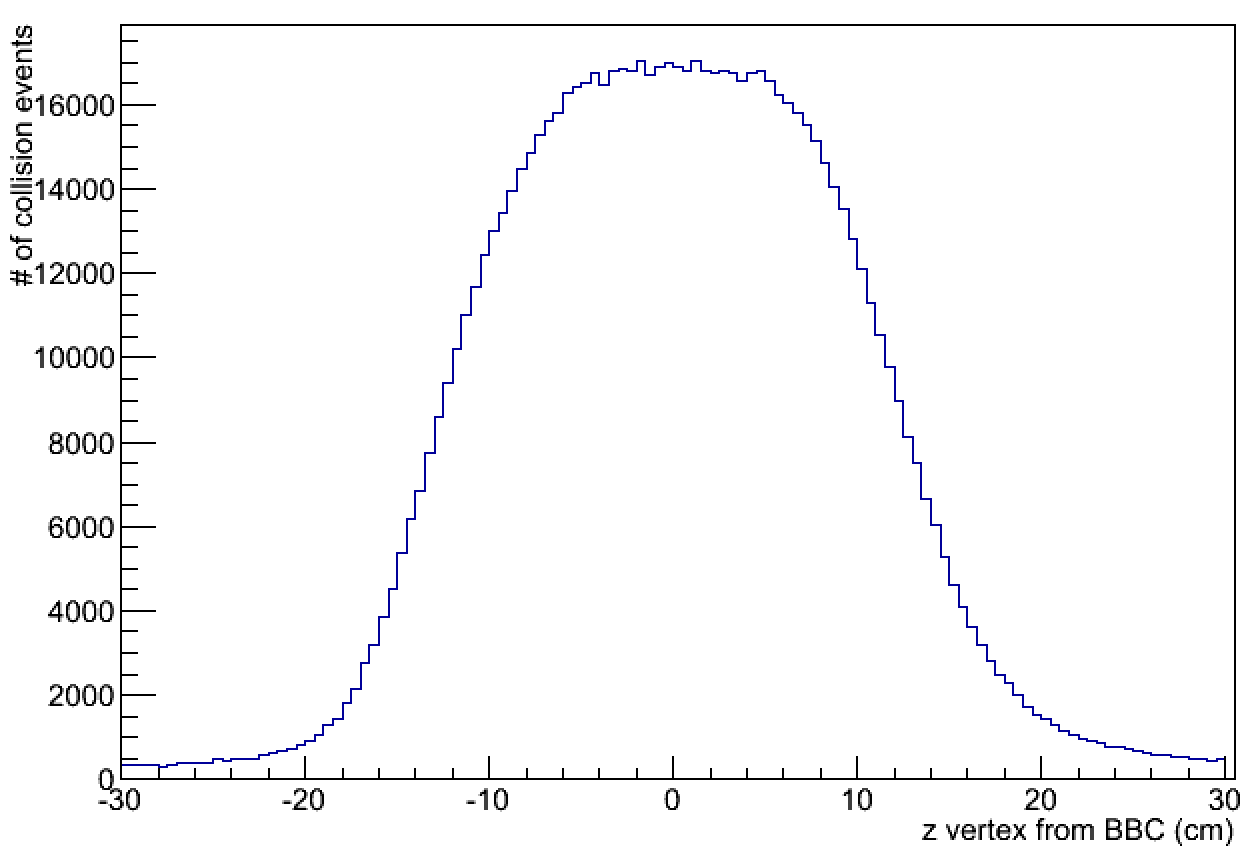
\includegraphics[width=0.65\linewidth]{figs/bbc_z_vertex_dist.png}
\caption{The distribution of BBC calculated z-vertex positions for events in p+Au 200 GeV. There are more events between -10 and 10 cm because of the BBC narrow trigger.}\label{fig:bbc_z_vtx_dist}

\end{center}
\end{figure}


%\section{Event Reconstruction and Characterization}
%[not sure about this section]
%\subsection{Central Arm Tracking}
%\begin{figure}
%\begin{center}
%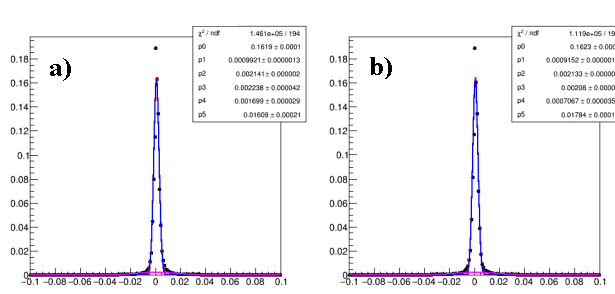
\includegraphics[scale=0.35]{figs/pc3dphi.png}
%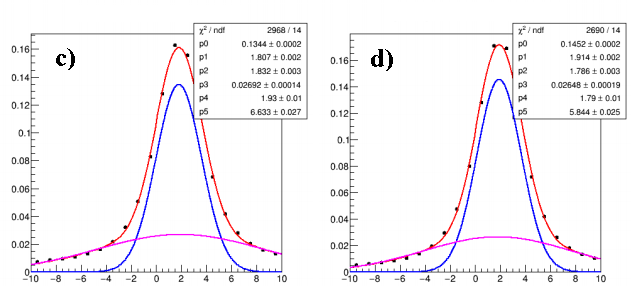
\includegraphics[scale=0.35]{figs/pc3dz.png}
%\end{center}
%\caption{TBA}
%\end{figure}
%\subsection{CNT Tracks Simulation}
%\subsection{Centrality Determination}
%\subsection{Vertex Determination}
%\begin{figure}
%\begin{center}
%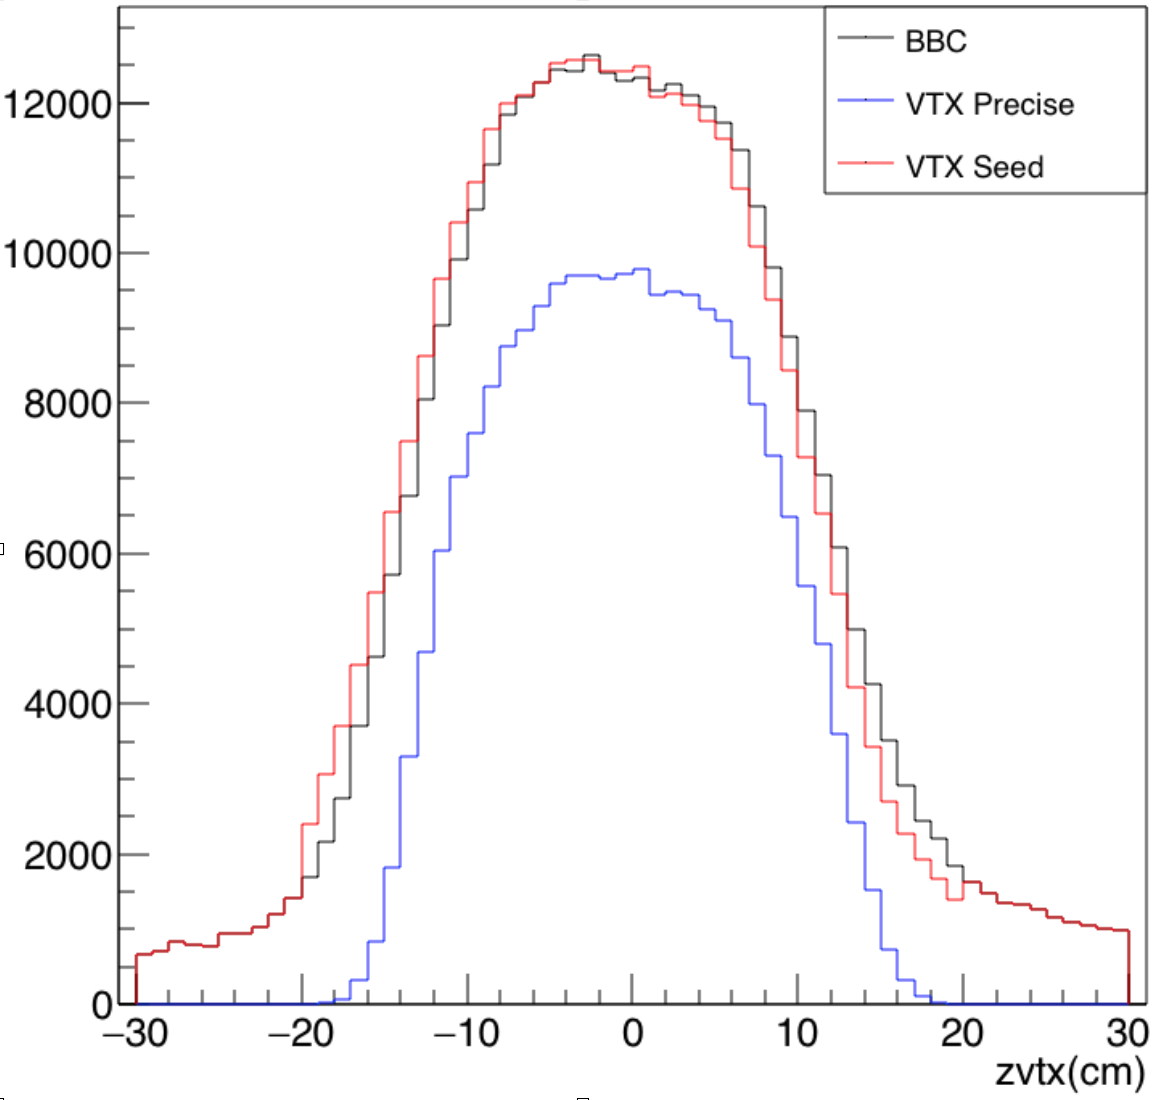
\includegraphics[scale=0.35]{figs/zvtx_distributions.png}
%\end{center}
%\caption{TBA}
%\end{figure}



%\section{Run15 pAu Dataset}
%\subsection{Beam Geometry Effects}
%\begin{figure}
%\begin{center}
%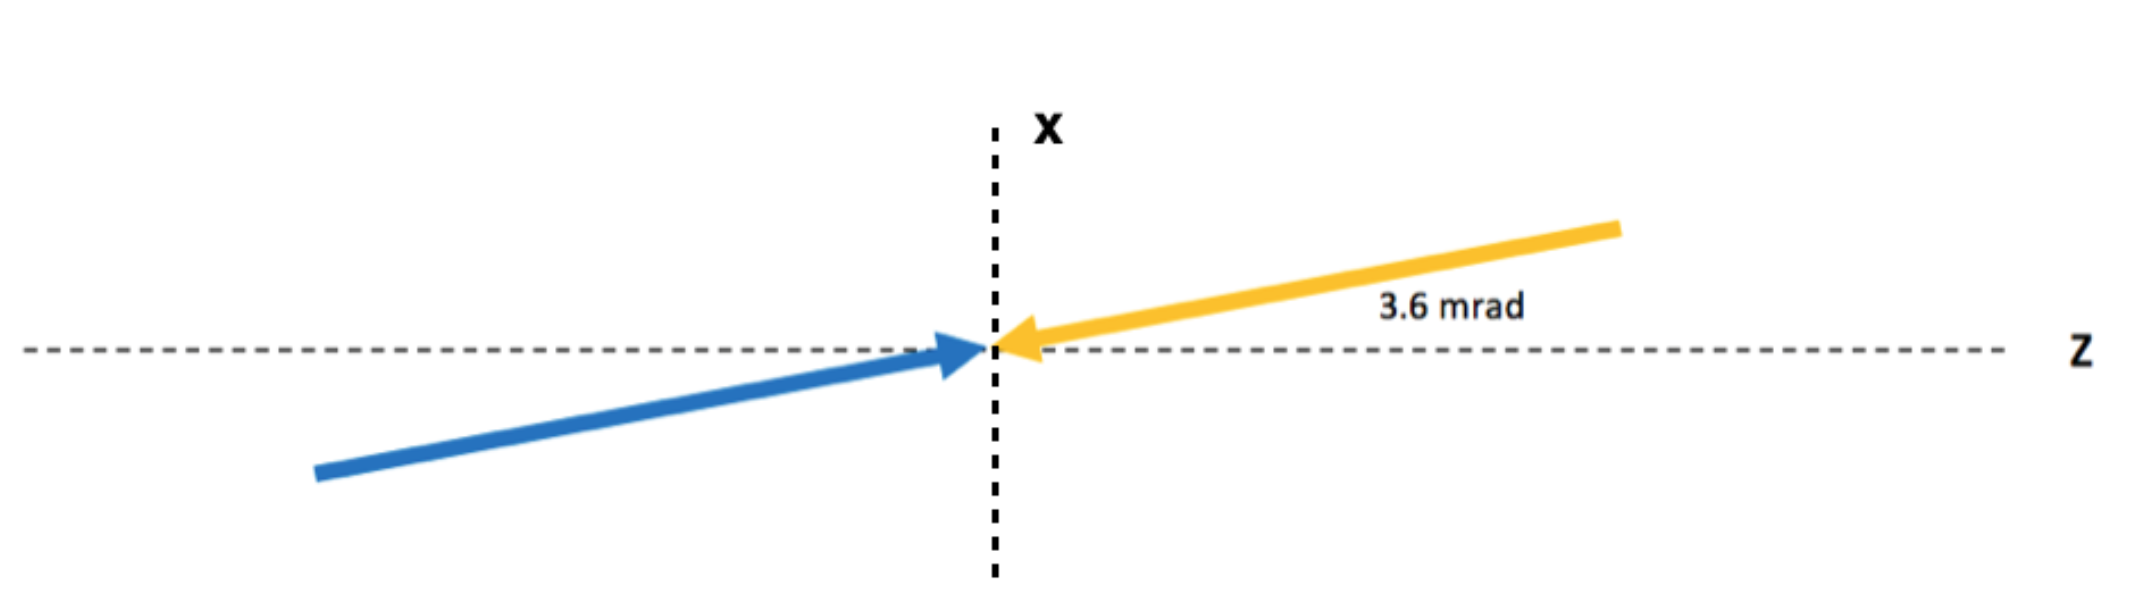
\includegraphics[width=0.65\linewidth]{figs/beam_angle.png}
%\caption{A vector diagram illustrating the yellow and blue beam angle.}
%\end{center}
%\end{figure}


